\section{Capitolo 3}
\underline{Le funzioni usate nei codici seguenti sono in fondo al capitolo}
\subsection{Esercizio 1}
Una matrice \( L \in M_{n \times n} \) si dice triangolare inferiore se \( l_{i,j}=0, \forall i<j \) con \(i,j = 1...n \) ed \( l_{i,j} \in L \).
\\
Date due matrici triangolari inferiori \( L,K \in M_{n \times n} \) la loro somma sar\'a di nuovo una matrice traingolare inferiore \( N \in M_{n \times n} \):
\[
 \forall i<j, \hspace{5pt} l_{i,j} + k_{i,j} = 0 + 0 = 0. 
\]
\\
Una matrice \( U \in M_{n \times n} \) si dice triangolare superiore se \( u_{i,j}=0, \forall i>j \) con \(i,j = 1...n \) ed \( u_{i,j} \in U \).
Date due matrici triangolari superiori  \( U,W \in M_{n \times n} \)  il loro prodotto  \( Z \in M_{n \times n} \):
\[
z_{i,j} = \sum_{k=1}^n u_{i,k} w_{k,j}, \hspace{35pt} \forall i,j \in [1,..,n].
\]
sar\'a di nuovo una matrice triangolare superiore, dal momento che 
\[
z_{i,j} =  \sum_{k=1}^n u_{i,k} w_{k,j} =  \underbrace{ \sum_{k=1}^{i-1} u_{i,k} w_{k,j} }_\text{=0 per k<i}  + \sum_{k=i}^n u_{i,k} w_{k,j} = \sum_{k=i}^n u_{i,k} w_{k,j}.
\]
Dal momento che in quest'ultimo termine abbiamo \( k \geq i \) se \( i>j \) allora \( k>j \), da cui la definizione di matrice triangolare superiore.

\subsection{Esercizio 2}
Se $U,W \in M_{n \times n}$ sono matrici triangolari superiori a diagonale unitaria si ha che gli elementi diagonali della matrice $Z=UW$ saranno calcolati come
\[
z_{i,i} = \sum_{k=i}^{i} u_{i,i}w_{i,i} = 1 \cdots 1 = 1.
\]
Quindi, riallacciandosi alla dimostrazione dell'esercizio \textbf{3.1} si ha che la matrice $Z$ \'e triangolare superiore a diagonale unitaria.
$symbol$

\subsection{Esercizio 3}
Sia $A \in M_{n \times n}$ una matrice triangolare superiore non singolare.\\
Se $A$ \'e invertibile allora pu\'o essere scritta come $A=D(\mathit{I_n}+U)$ dove $D$ \'e una matrice diagonale per cui vale $diag(D)=diag(A)$, $\mathit{I_n}$ \'e la matrice identit\'a ed $U$ \'e una matrice triangolare strettamente superiore ($diag(U)=0$).\\
Per le propriet\'a delle matrici triangolari strettamente superiori si ha che $U^n = 0$ (ovvero che la matrice $U$ \'e nilpotente), mentre per le propriet\'a delle matrici diagonali si ha che $D^{-1}$ \'e ancora una matrice diagonale.
\\
Volendo provare che $A^{-1}=(\mathit{I_n}+U)^{-1}D^{-1}$ espandiamo in serie $ (\mathit{I_n}+U)^{-1}$:
\[
(\mathit{I_n}+U)^{-1}=\mathit{I_n}-U+U^2-...+(-1)^{n-1}U^{n-1}.
\]
Essendo questa una serie di somme e prodotti di matrici triangolari superiori la matrice inversa $A^{-1}$ sar\'a in generale una matrice triangolare superiore.
\subsection{Esercizio 4}
L'eliminazione nella prima colonna richiede $n$ somme ed $n$ prodotti per $n-1$ righe, quindi in totale $(n+n)(n-1) = 2n(n-1)$ \texttt{flops}. L'eliminazione della seconda richiede $n-1$ somme ed $n-1$ prodotti per $n-2$ righe, quindi in totale $[(n-1)+(n-1)](n-2) = 2(n-1)(n-2)$ \texttt{flops}.\\
Procedendo per induzione si ha che il numero totale di operazioni \'e
\[
\sum_{i=0}^{n} 2(n-i)(n-i+1). \hspace{50pt} (1)
\]
Operando la sostituzione $y \doteq n-i+1$ si ha che la (1) diviene :

\[
2 \sum_{j=0}^{n-1} j(j-1) = 2 \sum_{j=0}^{n-1}j^2 + j = 2 ( \frac{1}{3}n^3 - \frac{1}{3}n)
\]
Asintoticamente quindi proprio $\frac{2}{3}n^3$ \texttt{flops}.


\newpage
\subsection{Esercizio 5}
\begin{flushleft}
L'algoritmo di fattorizzazione LU con pivoting parziale da noi implementato è il seguente:
\lstinputlisting[language=matlab]{cap_3/factLUP.m}
è possibile vedere il funzionamento di questa function nell'esercizio 14 a pagina \pageref{es314}.
\end{flushleft}
\subsection{Esercizio 6}
\lstinputlisting[language=Matlab]{cap_3/solveLinearLUP.m}

\subsection{Esercizio 7}
Sia $\mathbf{v} \in \mathbb{R}^n| \mathbf{v} \neq \mathbf{0}$ e $A \in M_{n \times n}$.
$A$ si dice sdp (simmetrica definita positiva) se \'e simmetrica ($A$=$A^T$) e se $\mathbf{v}^TA\mathbf{v} > 0.$
Equivalentemente una matrice si dice sdp se \'e simmetrica ed i suoi autovalori sono $> 0.$
Inoltre una matrice $B \in M_{n \times n}$ si dice nonsingolare se $\det{B} \neq 0.$
\\
Dal momento che il polinomio caratteristico \'e invariante per similitudine le matrici quadrate $A$ ed $A^T$ hanno gli stessi autovalori.
Inoltre le matrici $A^TA$ ed $AA^T$ sono simmetriche.
Vale poi $\det{(A^TA)} = \det{(AA^T)} = \det{A}\det{A^T} = (\det{A})^2.$

finisco stase

\subsection{Esercizio 8}
Se $A \in M_{m \times n}$ con $m \geq n = rank(A)$ allora diremo che $A$ ha rango massimo.
\\
Questo comporta che la matrice sia invertibile, ovvero che il suo determinante $\det(A) \neq 0$. La matrice \'e quindi nonsingolare e di conseguenza simmetrica definita positiva, dalla dimostrazione dell'esercizio \textbf{3.7}.
\subsection{Esercizio 9}
Si ha ovviamente che 
\[
A = \frac{1}{2}(A+A^T) + \frac{1}{2}(A-A^T)=\frac{1}{2}A + \frac{1}{2}A^T + \frac{1}{2}A - \frac{1}{2}A^T
\]
\\
Definendo $A_s \doteq \frac{1}{2}(A+A^T)$ si mostra come $A_s = A_s^T$ infatti
\[
\frac{1}{2}(A+A^T) = [ \frac{1}{2}(A+A^T)]^T = \frac{1}{2}(A+A^T)^T = \frac{1}{2}(A^T+(A^T)^T) = \frac{1}{2}(A+A^T)^T.
\]
\\
Da cui $A_s$ \'e detta parte \textbf{simmetrica} di $A$.
\\
Definendo $A_a \doteq \frac{1}{2}(A-A^T)$ si mostra come $A_a = -A_a^T$ infatti
\[
\frac{1}{2}(A-A^T) = -\frac{1}{2}(A-A^T)^T = -\frac{1}{2}(A^T-(A^T)^T) = -\frac{1}{2}(A^T-A) = \frac{1}{2}(A-A^T).
\]
Da cui $A_a$ \'e detta parte \textbf{antisimmetrica} di $A$.
\\
Dato poi un generico vettore $\mathbf{x} \in \mathbf{R}^n$ si ha che $\mathbf{x}^TA\mathbf{x} = \mathbf{x}^TA_s\mathbf{x}$ infatti
\[
\mathbf{x}^TA\mathbf{x} = \mathbf{x}^T(A_s + A_a)\mathbf{x} = \mathbf{x}^TA_s\mathbf{x} + \mathbf{x}^TA_a\mathbf{x} = \frac{1}{2}(\mathbf{x}^TA\mathbf{x} + \mathbf{x}^TA^T\mathbf{x}) + \frac{1}{2}(\mathbf{x}^TA\mathbf{x} - \mathbf{x}^TA^T\mathbf{x}).
\]
Analizzando l'ultimo termine $\frac{1}{2}(\mathbf{x}^TA\mathbf{x} - \mathbf{x}^TA^T\mathbf{x})$ si nota come
\[ \frac{1}{2}(\mathbf{x}^TA\mathbf{x} - \mathbf{x}^TA^T\mathbf{x}) = \frac{1}{2}(\mathbf{x}^TA\mathbf{x} - (A\mathbf{x})^T\mathbf{x})=0
\]
\\
dal momento che, definendo $A\mathbf{x}=\mathbf{y}$ si ha $\mathbf{x}^T\mathbf{y}= \mathbf{y}^T\mathbf{x}.$
Da cui la tesi.

\subsection{Esercizio 10}
L'algoritmo esegue $i-1$ somme di due prodotti, una sottrazione ed una divisione per un costo totale di $2(i-1)+2$ \texttt{flops}. Essendo la matrice triangolare, per ogni colonna eseguir\'a il calcolo $n-i$ volte.
\\
Quindi
\[
\sum_{i=1}^{n} 2i(n-i) = 2(n \sum_{i=1}^{n}i - \sum_{i=1}^{n} i^2) = 2n\frac{n(n+1)}{2} - 2\frac{n(n+1)(2n+1)}{6} = n^3 + n^2 - \frac{2n^3 + 3n^2 + n}{3} = \frac{n^3}{3} - \frac{n}{3} \approx \frac{n^3}{3}.
\]

\subsection{Esercizio 11}
\lstinputlisting[language=Matlab]{cap_3/es11/fattorizzaLDLt.m}
\subsection{Esercizio 12}
\begin{flushleft}
Supponendo che in ingresso si abbiano le matrici di fattorizzazione $LDL^T$ di una qualsiasi matrice $M \in \mathbb{R}^{n\times n}$ SDP, rispettivamente:
\begin{itemize}
    \item L matrice triangolare inferiore a diagonale unitaria
    \item D matrice diagonale con elementi diagonali positivi
\end{itemize}
e b vettore dei termini noti, è possibile scrivere la function linLDL che risolve sistemi lineari:
\lstinputlisting[language=matlab]{cap_3/linLDLT.m}
\end{flushleft}
\subsection{Esercizio 13}
\begin{flushleft}
Per verificarlo abbiamo usato il seguente codice MatLab:
\lstinputlisting[language=Matlab]{cap_3/es13/es13.m}
Che restituisce l'output:
\begin{lstlisting}[language=matlab, basicstyle = \small]
A1 =
     1     1     1     1
     1     2     2     2
     1     2     3     3
     1     2     3     4
L1 =
     1     0     0     0
     1     1     0     0
     1     1     1     0
     1     1     1     1
D1 =
     1     0     0     0
     0     1     0     0
     0     0     1     0
     0     0     0     1
     
A2 =
     1     1     1     1
     1     2     2     2
     1     2     3     3
     1     2     3     2
Error using factLDLT (line 14)
[Errore] La matrice non e' SDP
Error in es13 (line 6)
[L2,D2] = factLDLT(A2) 
\end{lstlisting}
L'output è molto chiaro, la seconda matrice $A_{2}$ non può essere fattorizzata $LDL^T$ di conseguenza non è $SDP$.
\end{flushleft}


\subsection{Esercizio 14}
\label{es314}
\begin{flushleft}
Nel primo caso abbiamo usato la matrice $A\in M^{3\times 3}$ con elementi:
\[ 
A =
\begin{pmatrix}
    0 & -3 &  8 \\
   -1  &  8  &  7 \\
    1  &  3  &  0 \\
\end{pmatrix}
\]
e il vettore dei termini noti $b\in \mathbb{R}^3$ con valori:
\[
b = \begin{pmatrix}
    3.1416 \\
    1.1618 \\
    2.7183 \\
\end{pmatrix}
\]
Nel secondo caso abbiamo usato la matrice $A\in M^{3\times 3}$ con elementi:
\[ 
A =
\begin{pmatrix}
    14 & 5 &  2 \\
    5 &  8  &  1 \\
    2  &  1  &  4 \\
\end{pmatrix}
\]
e il vettore dei termini noti $b\in \mathbb{R}^3$ con valori:
\[
b = \begin{pmatrix}
    3.1416 \\
    1.1618 \\
    2.7183 \\
\end{pmatrix}
\]
Usando il codice MatLab sottostante è possibile risolvere questi 2 esempi:
\lstinputlisting[language=Matlab]{cap_3/es14/es14.m}
Il codice sopra restituisce l'output:
\begin{figure}[H]
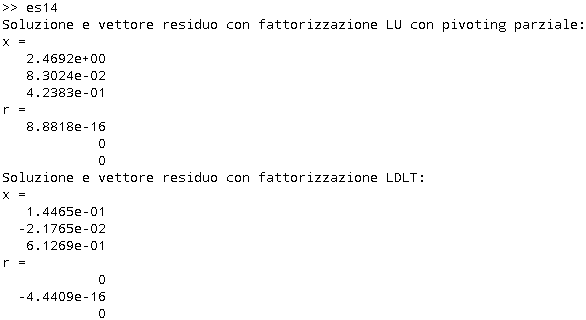
\includegraphics[left, width=300px]{cap_3/es14/es314.png}
\end{figure}
\end{flushleft}
\subsection{Esercizio 15}
\begin{flushleft}
\lstinputlisting[language=Matlab]{cap_3/es15/es15.m}
Il codice MatLab sopra restituisce in output:
\begin{lstlisting}[language=matlab, basicstyle = \small]
ans =
    101.000000000000e+000
ans =
    101.000000000000e+000
Warning: Matrix is close to singular or badly scaled.
Results may be inaccurate. RCOND =  9.801980e-21. 
> In cond (line 46)
  In es15 (line 7) 
ans =
    102.020202020202e+018
\end{lstlisting}
Analiticamente abbiamo che $\rVert A \rVert_{\infty} = \rVert A \rVert_1 = 101$, come \'e possibile verificare attraverso l'istruzione norm di Matlab.
Per quanto riguarda il calcolo del numero di condizionamento $k_{\infty}(A)$ abbiamo che, andando a calcolare l'inversa, gli elementi della matrice crescono di 2 ordini di grandezza per ogni riga, arrivando ad avere valori prossimi a $10^{18}$. Questo implica che $\rVert A^{-1} \rVert_{\infty}>10^{20}$ per cui possiamo affermare che il problema \'e malcondizionato.
La verifica con l'istruzione cond di Matlab restituisce un warning in cui avverte che $RCOND=9.801980e-21$, confermando quanto appena detto.
\end{flushleft}
\subsection{Esercizio 16}
\lstinputlisting[language=Matlab]{cap_3/es16/es16.m}

\subsection{Esercizio 17}
\begin{flushleft}
L'algoritmo di fattorizzazione QR, mediante metodo di householder, da noi implementato è il seguente:
\lstinputlisting[language=matlab]{cap_3/factQRH.m}
è possibile vedere il funzionamento di questa function nell'esercizio 19 a pagina \pageref{es319}.
\end{flushleft}
\subsection{Esercizio 18}
\lstinputlisting[language=Matlab]{cap_3/solveQR.m}

\newpage
\subsection{Esercizio 19}
\label{es319}
\begin{flushleft}
Il codice usato è:
\lstinputlisting[language=Matlab]{cap_3/es19/es19.m}
che ha generato questo risultato:
\begin{figure}[h]
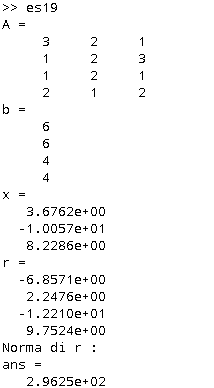
\includegraphics[left, width=300px]{cap_3/es19/es319}
\end{figure}
\end{flushleft}

\subsection{Esercizio 20}
Risolviamo il sistema di equazioni non lineari applicando il metodo di Newton.
La funzione data è \[F(x_1, x_2)= \begin{cases}x_2-cos(x_1)\\ x_1x_2 -1/2\end{cases}\]
Vogliamo trovare $F(x_1, x_2)=0$ partendo da $x_1(0) = 1\mbox{, } x_2(0) = 1$\\
Troviamo quindi il Jacobiano della funzione: \( J=\begin{pmatrix} sin(x_1) & 1  \\\ x_1 & x_2 \end{pmatrix} \)\\
Applicando il metodo di Newton si va a risolvere:
$\begin{cases} J_F(\underline{x}^{(k)})\underline{d}^{(k)}=-F(\underline{x}^{(k)}) \\ \quad \underline{x}^{(k+1)}=\underline{x}^{(k)}+\underline{d}^{(k)} \end{cases}$\\
Troviamo quindi: $x_1 = 0.6100 \mbox{ e } x_2 =0.8196$

Il codice matlab per il calcolo del minimo è:
\lstinputlisting[language=Matlab]{cap_3/es20/es20.m}

Il codice matlab per la risoluzione di sistemi di equazioni non lineari mediante Newton è:
\lstinputlisting[language=Matlab]{cap_3/NewtonNL.m}

\begin{tabular}{l|c|r}
i & $x_1,x_2$ & norma dell'incremento \\
\hline
1 & 0.7458, 0.7542 & 0.5001 \\
2 & 0.5531, 0.8653 & 0.3145 \\
3 & 0.6042, 0.8241 & 0.0929 \\
4 & 0.6100, 0.8197 & 0.0102 \\
5 & 0.6100, 0.8196 & 0.00013 \\ 


\end{tabular}

\subsection{Esercizio 21}
Un punto stazionario $(\hat{x_1}, \hat{x_2})$ è tale per cui $J(\hat{x_1},\hat{x_2})=0$. Si ottiene quindi il sistema non lineare:
$$F(\underline{x})=\underline{0}\mbox{ con }F=\begin{pmatrix}\frac{\partial f}{\partial x_1}\\\frac{\partial f}{\partial x_2}\end{pmatrix}=\begin{pmatrix}4x_1^3+2x_1+x_2\\x_1+2x_2-2\end{pmatrix}.$$
Troviamo il Jacobiano della funzione: \( J=\begin{pmatrix} 12x_1^2+2 & 1  \\\ 1 & 2 \end{pmatrix} \)\\

Troviamo quindi $$\min{f(x_1,x_2)}\approx -0.2573\mbox{ in }(0.4433, -1.2217).$$


Il codice matlab per il calcolo del minimo è:
\lstinputlisting[language=Matlab]{cap_3/es21/es21.m}

\newpage
\subsection{Funzioni MatLab Usate}
\label{functcap3}
\begin{flushleft}
\subsubsection{Fattorizzazioni}
\begin{itemize}
    \item \texttt{Fattorizzazione LU con pivoting parziale}
\lstinputlisting[language=Matlab]{cap_3/factLUP.m}
    \item \texttt{Fattorizzazione LDLT}
\lstinputlisting[language=Matlab]{cap_3/factLDLT.m}
    \item \texttt{Fattorizzazione QR mediante metodo di Householder}
\lstinputlisting[language=Matlab]{cap_3/factQRH.m}
\end{itemize}
\subsubsection{Function per la risoluzione sistemi lineari}
\begin{itemize}
    \item \texttt{Calcolo matrice trinagolare inferiore}
\lstinputlisting[language=Matlab]{cap_3/triInf.m}
    \item \texttt{Calcolo matrice trinagolare superiore}
\lstinputlisting[language=Matlab]{cap_3/triSup.m}
    \item \texttt{Calcolo diagonale principale}
\lstinputlisting[language=Matlab]{cap_3/triSup.m}
\end{itemize}
\subsubsection{Risoluzione sistemi lineari, sovradeterminati e non lineari}
\begin{itemize}
    \item \texttt{Risoluzione sistema lineare con matrice matrice dei coefficienti fattorizzata LUP}
\lstinputlisting[language=Matlab]{cap_3/linLUP.m}
    \item \texttt{Risoluzione sistema lineare con matrice matrice dei coefficienti fattorizzata LDLT}
\lstinputlisting[language=Matlab]{cap_3/linLDLT.m}
    \item \texttt{Risoluzione sistema lineare sovradeterminato con matrice dei coefficienti fattorizzata QRH}
\lstinputlisting[language=Matlab]{cap_3/solveQRH.m}
    \item \texttt{Risoluzione sistema non lineare con metodo di Newton}
\lstinputlisting[language=Matlab]{cap_3/nonLinearNewton.m}
\end{itemize}
\end{flushleft}